%% ID: trailer_truck
%% TITLE: Trailer truck
%% TYPE: question
%% QUESTIONTYPE:  numerical
%% CONCEPTS: forces, moments, newtoni
%% VIDEOS: 
%% LEVEL: 3
%% TOPIC: mechanics/statics
%% ORDER: 9

\begin{problem}[A1986PIQ2a] %balancing moments
%changed to not be multiple choice and to not have diagram in question
{\question{A trailer towed by a truck has a length \value{l}{20}{m} and has a mass \value{M}{3000}{kg} evenly distributed along that length. There is a crate of mass \value{m}{2000}{kg} sitting on the trailer at a distance \value{x}{5}{m} from the back of the trailer. The trailer has a set of wheels at one end and sits on top of the back of the truck's carriage at the other. Assuming \value{g}{10}{m\,s\sup{-2}}, find the magnitude \vari{F} of the contact force between the carriage and the trailer.}}
{\textit{Adapted with permission from UCLES, A Level Physics, June 1989, Paper 1, Question 2.}}
{\answer{\valuedef{F}{20}{kN}}
\begin{figure} [h]
	\centering
	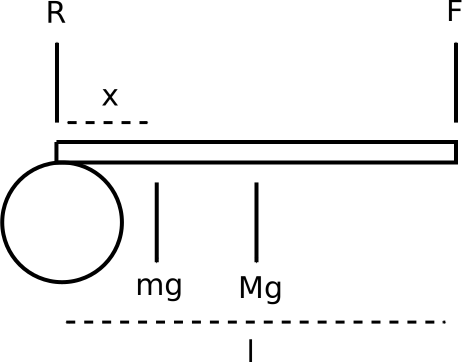
\includegraphics[width=0.4\textwidth]{../../../figures/Statics_trailer.svg}
	\caption{} \label{fig:Statics_trailer}
\end{figure}
The diagram in Figure \ref{fig:Statics_trailer} shows that we have two unknown forces: the normal reaction force \vari{N} at the back wheels and the normal reaction force \vari{F} on the trailer from the carriage of the truck. However, we only want the latter. We know the trailer is in equilibrium so, by taking moments about the back wheels, we find
\begin{equation*}
lF-\frac{1}{2}lMg-xmg=0	
\end{equation*}
\begin{equation*}
lF=\frac{1}{2}lMg+xmg	
\end{equation*}
\begin{equation*}
F=\frac{Mg}{2}+\frac{xmg}{l}	
\end{equation*}
And, putting in the numbers from the question,
\begin{equation*}
F=\frac{3000\times 10}{2}+\frac{5\times 2000\times 10}{20}=15000+5000=20000\textrm{ N}	
\end{equation*}
}
\end{problem}